\documentclass[12pt]{article}
\usepackage{lingmacros}
\usepackage{tree-dvips}
\usepackage[utf8]{inputenc}
\usepackage[russian]{babel}
\usepackage{amsmath,amssymb}
\usepackage{multirow}
\usepackage{hyperref}
\usepackage{caption}
\usepackage{tabularx}
\usepackage{enumitem}

\usepackage{graphicx}
\graphicspath{ {./images/} }

\begin{document}

\section*{Дефиниции}

\section*{Задачи}

\subsection*{Лесни}
\subsubsection*{Задача 1.1}
Да се докаже, че броят на върховете от нечетна степен в граф е четно число.
\subsubsection*{Задача 1.2}
Да се докаже, че във всеки граф има поне два върха с еднаква степен.
\subsubsection*{Задача 1.3 - Записки на Ангел Димитриев}
Нека $G = (V, E)$ е граф. Нека за всяко $v \in V$ е вярно, че $d(v) \geq 2$. Да се докаже, че в $G$ има цикъл. 
\subsubsection*{Задача 1.4 - Записки на Ангел Димитриев}
6 тенисисти играят в турнир (всеки срещу всеки).  Да се докаже, че съществуват двама, за които е вярно, че всеки от останалите е загубил от поне един от двамата.
\subsubsection*{Задача 1.5 - Записки на Ангел Димитриев}
Нека $G$ е неориентиран граф и $n$ е четно. Нека всички върхове са от степен $\frac{n}{2} + 1$. Да се докаже, че в $G$ има цикъл с дължина 3.
\subsubsection*{Задача 1.5 - Домашно - Информатика - 2021/2022}
\paragraph*{}
Игралното поле на Minesweeper се състои от клетки. В някои клетки има мини. Останалите клетки са свободни. Допълнението на игрално поле се получава, като поставим мини в свободните клетки и премахнем мините от клетките, които дотогава са били заети.
\begin{center}
    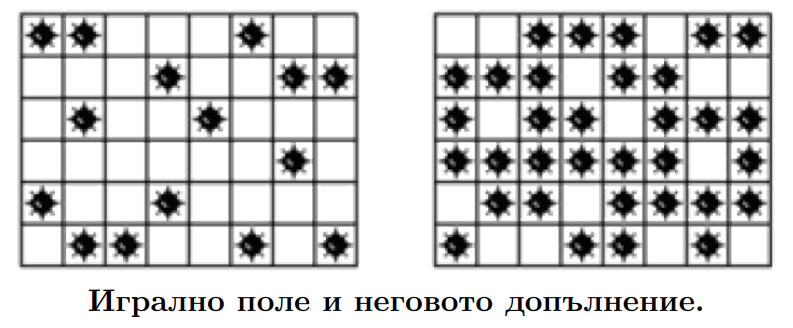
\includegraphics[scale = 0.5]{minesweeper-1}
\end{center}
\paragraph*{}
Във всяка празна клетка записваме цяло неотрицателно число — броя на съседните клетки, заети от мини. (В клетките с мини не пишем числа.) Съседни са тези клетки, които притежават общ ръб или общ връх. Например всяка клетка, която не е по контура на игралното поле, има осем съседни клетки.
\paragraph*{}
Забележителен факт е, че всяко игрално поле и неговото допълнение имат еднакъв сбор от числата, записани в клетките. Например за показаното тук игрално поле този сбор е 75.
\begin{center}
    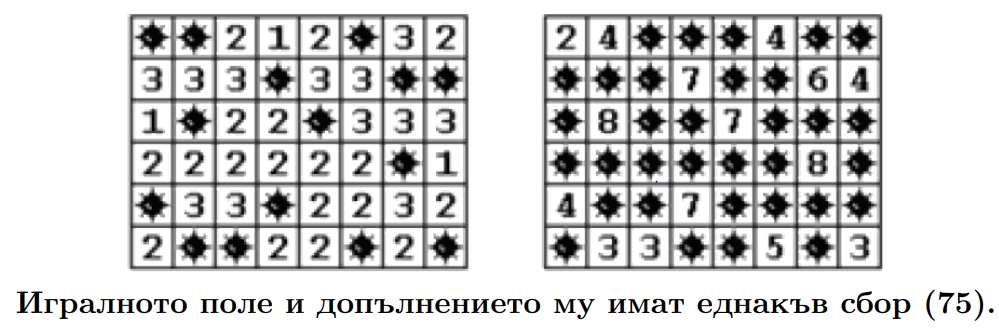
\includegraphics[scale = 0.5]{minesweeper-2}
\end{center}
\paragraph*{}
Още по -интересно е, че това свойство важи за всяка релация на съседство между клетките.
\begin{itemize}
    \item Разгледайте следната релация на съседство: две клетки са съседни само ако имат общ ръб. Така всяка клетка, която не е по контура на игралното поле, има четири съседни клетки. За разположението на мините от примера по -горе проверете, че равенството на сборовете важи и за тази релация на съседство.
    \item С теорията на графите докажете равенството на сборовете. Доказателството трябва да важи за всяко игрално поле и всяка симетрична релация на съседство между клетките. 
\end{itemize}
\subsubsection*{Задача 1.2 - изпит - КН - 2019/2020}
\paragraph*{}
На петте острова Гренландия, Ирландия, Исландия, Мадагаскар и Ямайка има общо сто града — $T_1, T_2, ..., T_{100}$. Между някои от градовете има едно или повече шосета, а между други двойки градове няма нито едно шосе. Градът $T_1$ се намира на остров Гренландияи е край на точно едно шосе. Градът $T_{100}$ е край на точно точно три шосета, а всеки от другите градове е край на точно четири шосета. Вярно ли е, че $T_1$ и $T_{100}$ се намират на един остров?
\paragraph*{}
\emph{Очевидно може да има шосета само между два града на един и същи остров.}
\subsubsection*{Задача 1.3 - изпит - КН - 2019/2020}
\paragraph*{}
В краен неориентиран граф без примки е избран неизолиран връх $v_0$. Известно е, че има единствен най-дълъг прост път и той е с начало $v_0$. Докажете, че краят му (различен от $v_0$) е от нечетна степен.
\subsubsection*{Задача 1.4 - Записки на Ангел Димитриев}
Да се докаже, че в граф с поне 6 върха има 3-клика или 3-антиклика.
\subsubsection*{Задача 1.5 - Записки на Ангел Димитриев}
Да се премсетне броя на кликите и антикликите в $K_n$.
\subsubsection*{Задача 1.6 - Записки на Ангел Димитриев}
Да се докаже, че в дърво има поне два връха от степен 1. 
\subsubsection*{Задача 1.7 - Записки на Ангел Димитриев}
Да се докаже, че $G$ e дърво $\iff$ между всеки два върха има точно един път.
\subsubsection*{Задача 1.8 - Записки на Ангел Димитриев}
Нека $T = <V, E>$ е дърво. Нека за всяко $v \in V$ $d(v) \in \{ 1, 4\}$. Да се докаже, че $n \equiv 2 (mod \; 3)$.
\subsubsection*{Задача 1.9 - Записки на Ангел Димитриев}
Нека $G = <V, E>$ е граф. Да се докаже, че броя на циклите в $G$ е $\geq |E| - |V| + 1$.
\subsubsection*{Задача 1.10 - Записки на Ангел Димитриев}
Нека $G = <V, E>$ е двуделен граф и $|V| \geq 5$. Да се докаже, че $\overline{G}$ не е двуделен.
\subsubsection*{Задача 1.11 - Записки на Ангел Димитриев}
Да се докаже, че сумата на степените на върховете от двата дяла на двуделния граф са равни.
\subsubsection*{Задача 1.12 - Записки на Ангел Димитриев}
Да се докаже, че двуделен граф с върхове, чиито степени са равни, има равни по-големина дялове.
\subsubsection*{Задача 1.13 - Записки на Ангел Димитриев}
Нека $G = <V, E>$ е граф. Нека $|V|$ е нечетно и всички върхове са от една и съща степен. Да се докаже, че $G$ не е двуделен. 
\subsubsection*{Задача 1.13 - Изпит КН - 2020}
Докажете или опровергайте, че съществува граф $G$ с 51 върха, такъв че $G$ и $\overline{G}$ са изоморфни.
\subsubsection*{Задача 1.14 - Изпит КН - 2020}
\paragraph*{}
Химик разполага с n вещества, които умее да превръща едно в друго с химични реакции. За всяко $i \in \{ 1, ..., n\}$ и за всяко $j \in \{ 1, ..., n \}$ е дадено $T(i, j)$ броят на начините за пряко превръщане на $i$-тото в $j$-тото вещество, където $T(i, j) \in \mathbb{N}$. Всички числа $T(i, j)$ се смятат за $\textbf{дадени}$. 
\paragraph*{}
Пряко превръщане означава превръщане, осъществено с помощта на точно една химична реакция. Съществуват обаче и косвени превръщания, всяко от които е поредица от две или повече химични реакции: едно вещество се превръща в друго с пряко превръщане, то се превръща в трето с пряко превръщане и така нататък до получаване на желаното крайно вещество.
\paragraph*{}
Забележете, че при тези условия е възможно едно вещество да бъде превръщано в себе си, при това по няколко начина. Нещо повече: ако превърнем i-тото вещество в самото него и после пак превърнем $i$-тото вещество в самото него, това е косвено превръщане с две междинни реакции.
\paragraph*{}
Отговорете на следния въпрос. При дадени $l$ и $m$, където $l, m \in \{ 1, ..., n \}$, по колко начина можем да превърнем вещество номер $l$ във вещество номер $m$ чрез точно $100$ междинни реакции?

\subsection*{По-забавни}
\subsubsection*{Задача 2.1 - Домашно - Информатика - 2021/2022}
Нека $G = (V, E)$ е граф. Нека $|V| = n$. Полагаме
\begin{equation*}
    k(v) = \frac{1}{d(v)} \displaystyle\sum_{u \in V, (u, v) \in E} d(u), \; \; \; \; \; \; D = \frac{1}{n}\displaystyle\sum_{v \in V} d(v), \; \; \; \; \; \; k = \frac{1}{n}\displaystyle\sum_{v \in V} k(v) 
\end{equation*}
\begin{itemize}
    \item Да се докаже, че $D \leq K$.
    \item Да се предложи практическо тълкуване на неравенството.
\end{itemize}

\subsubsection*{Задача 2.2 - Изпит - КН - 2021/2022}
Припомнете си алгоритъма на Дийкстра за намиране на най-къси пътища в тегловен граф с положителни тегла от връх s до всички останали върхове. Може ли да получим от него алгоритъм за най-дълги пътища в тегловен граф с положителни тегла от връх $s$ до всички останали върхове, ако обърнем неравенствата и заменим $\infty$ с $-\infty$ и заменим минимум с максимум? Става дума за следните промени.
\begin{enumerate}
    \item Инициализираме стойностите на върховете не с $\infty$, а с $-\infty$.
    \item Проверката за край на алгоритъма става ``ако извън множеството S няма връх със стойност, поголяма от $-\infty$, край''. В алгоритъма на Дийкстра тази проверка е ``ако извън множеството S няма връх със стойност, по-малка от $\infty$, край''.
    \item На всяка итерация избираме връх $x$, който да сложим в множеството от върхове $S$, като върхът с \textbf{максимална} стойност, който не е в $S$. В алгоритъма на Дийкстра избираме връх $x$, който да сложим в множеството от върхове $S$, като върхът с минимална стойност, който не е в $S$.
    \item При разглеждането на върховете от списъка на съседство на x обръщаме посоката на неравенството така: за всеки връх $y$ в списъка на съседство на $x$, ако стойността на $y$ е \textbf{по-малка} от стойността на $x$ плюс теглото на реброто $(x, y)$, присвояваваме на стойността на $y$ стойността на $x$ плюс теглото на реброто $(x, y)$. В алгоритъма на Дийкстра това присвояване се случва, ако стойността на $y$ е по-голяма от стойността на $x$ плюс теглото на реброто $(x, y)$.
\end{enumerate}
\subsubsection*{Задача 2.3 - Записки на Ангел Димитриев}
Да се преброят покриващите дървета в $K_{3, 3}$.

\section*{Решения}

\end{document}